\apendice{Especificación de diseño}

\section{Introducción}

En este apartado vamos a explicar que hemos usado para la resolución del problema en cuanto a herramientas de diseño.

Para la elaboración de los diagramas de paquetes y de clases hemos usado UML como metodología y el programa Astah para implementar los diagramas de clases.

Primero, hemos planeado un prototipo de diseño de cada una de las clases, que a medida que después las implementábamos las hemos ido completando, para que se correspondieran en lo que finalmente quedaba.



\section{Diseño de datos}

\subsection{Introducción}
En este punto vamos a hacer el diseño inicial de las clases de la aplicación y del diseño de paquetes en el que estarán contenidas.

\begin{figure}[h]
	\centering
	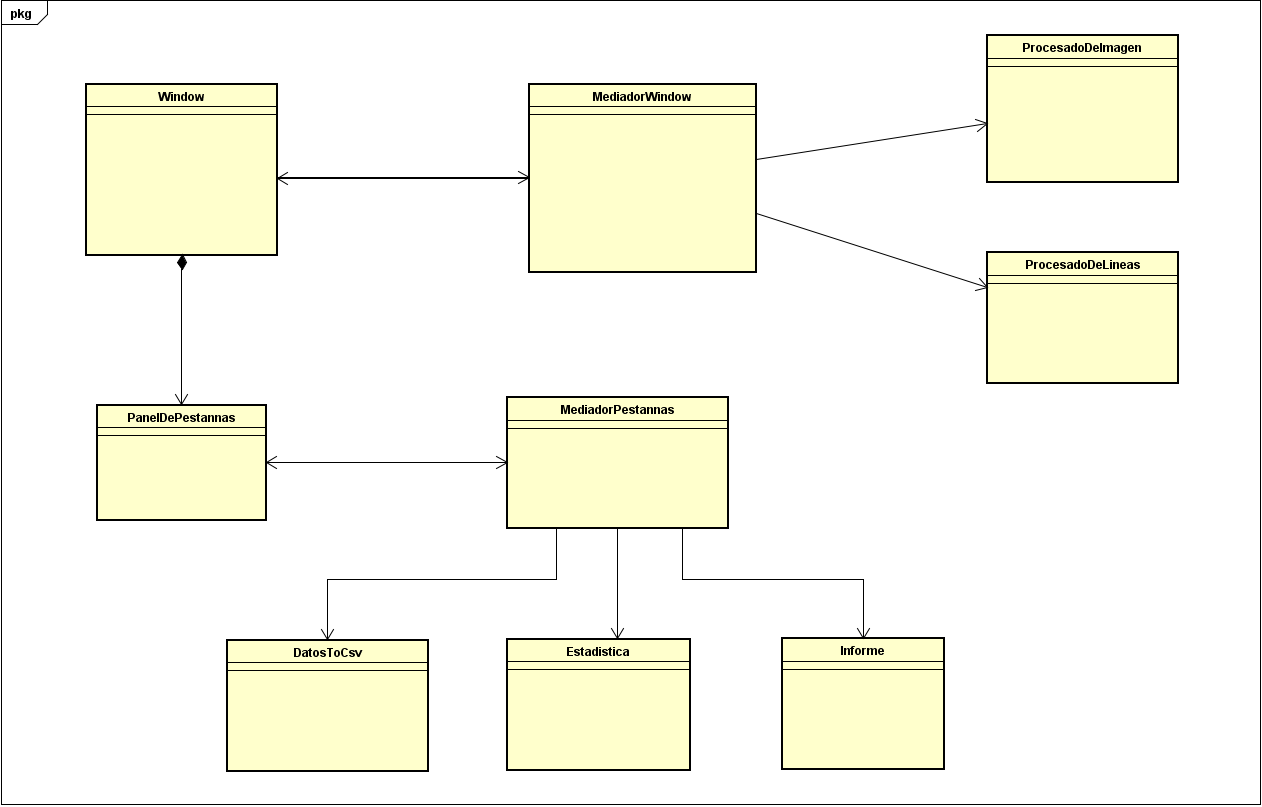
\includegraphics[width=.99\textwidth]{DiaClases}
	\caption{Diagrama de clases inicial}
	\label{fig:C.1.1}
\end{figure}
 


\subsection{Clases}
En esta parte vamos a hacer una breve descripción del contenido de cada clase y su función.

\begin{itemize}
	\item VentanaInicio: 
Esta clase simplemente hará de fachada entre la ejecución y el acceso a la aplicación real cuando hayamos elegido una imagen que procesar
	\item Window:
Esta clase contendrá la ventana principal, menús, el panel de pestañas y la imagen sobre la que dibujar.
	\item PanelDePestannas:
Esta clase contendrá la botonería y la interacción con la imagen a evaluar.
	\item MediadorPestannas:
Esta clase va a ser un mediador para las pestañas para deslocalizar código y complejidad.
	\item MediadorVentana:
En esta clase va ser un mediador entre la ventana principal y sus métodos para así reducir complejidad en la clase de ventana.
	\item ProcesadoDeImagen:
Esta clase contendrá el tratamiento que tiene que llevar la imagen para la extracción de características a evaluar.
	\item ProcesadoDeLineas:
Esta clase contendrá el procesado de las líneas obtenidas por el procesado de la imagen y el resultado final que obtendremos.
	\item Informe: 
Esta clase contendrá la generación del informe (Tabla) de estadísticas en formato \LaTeX para poder exportar fácilmente a un documento PDF.
	\item DatosToCsv:
Esta clase contendrá el paso de los datos que contiene la tabla a un documento en formato csv del que desde Excel podemos extraer fácilmente los datos.
	\item Estadistica: 
Esta clase contendrá el cálculo de los datos estadísticos y la clasificación de las líneas según su orientación.
\end{itemize}





\subsection{Diseño de la Interfaz}

\subsection{Primera versión}

Para el desarrollo de la interfaz gráfica pensé en una planificación espacial acorde con los elementos que esta contendría.
Un layout que seria muy adecuado podría ser un border layout pero como no existe en PyQt4 lo he tenido que simular gracias a apilar layouts de otros tipos.
Consiguiendo tener una botonería arriba del todo y dos columnas debajo claramente diferenciadas en la que en una estuviera la imagen que vamos a mostrar y en la otra las funcionalidades, como se ilustra en la imagen \ref{fig:5.8}.

\begin{figure}[h]
\centering
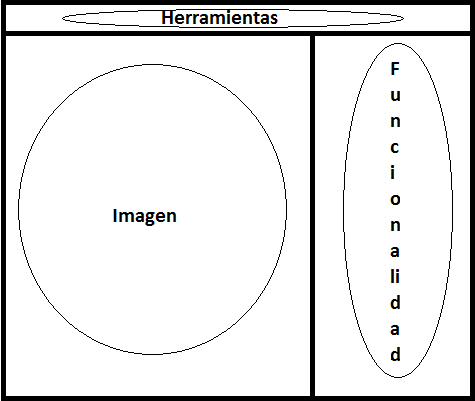
\includegraphics[width=0.65\textwidth]{disenoInter}
\caption{Diseño de la interfaz de usuario}
\label{fig:5.8}
\end{figure}

\subsection{Versión a evaluar}

En otro Sprint del proyecto lo que he usado han sido pestañas para así tener en la zona de funcionalidades los modos de trabajo de la aplicación claramente separados \ref{fig:5.9}.

\begin{itemize}
\item Detección líneas rojas.
\item Corrección y pintar líneas.
\item Automático.
\end{itemize}


\begin{figure}[h]
\centering
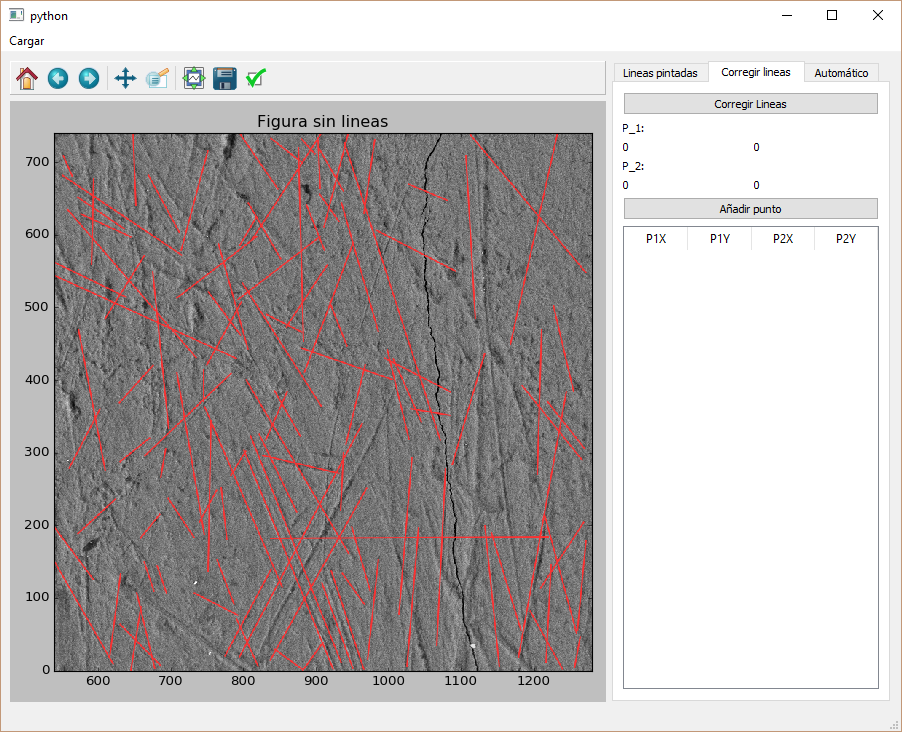
\includegraphics[width=0.65\textwidth]{disenoWi}
\caption{Diseño de la interfaz de usuario}
\label{fig:5.9}
\end{figure}
\subsubsection{Barra de herramientas}
Es una sección de la interfaz que nos va permitir de momento la carga de imágenes para su procesado \ref{fig:5.10}.
\begin{figure}[h]
\centering
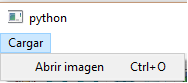
\includegraphics[width=0.65\textwidth]{BarraHerramientas}
\caption{Barra de herramientas de la aplicación}
\label{fig:5.10}
\end{figure}

\subsubsection{Barra de herramientas de la imagen}
Es una sección de la interfaz que nos permitirá manipular la imagen para realizar estas acciones \ref{fig:5.11}.

\begin{itemize}
\item Volver al principio. 
\item Retroceder un paso.
\item Avanzar un paso.
\item Desplazar la imagen.
\item Aumentar la región que seleccionemos.
\item Configurar la región, bordes, etc.
\item Guardar la imagen con su escala.
\item configurar el tamaño y numeración de los ejes.
\item Coordenadas actuales del ratón.
\item Niveles de color de los canales R G B del espacio RGB.
\end{itemize}

\begin{figure}[h]
\centering
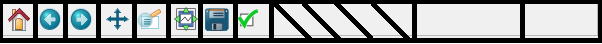
\includegraphics[width=0.95\textwidth]{toolbar}
\caption{Barra de herramientas de la imagen}\label{fig:5.11}
\end{figure}


\subsubsection{FigureCanvas de la imagen}
Es la región donde se muestra la imagen que va a ser ligeramente mas grande que la parte de las pestañas \ref{fig:5.12}.
\begin{figure}[h]
\centering
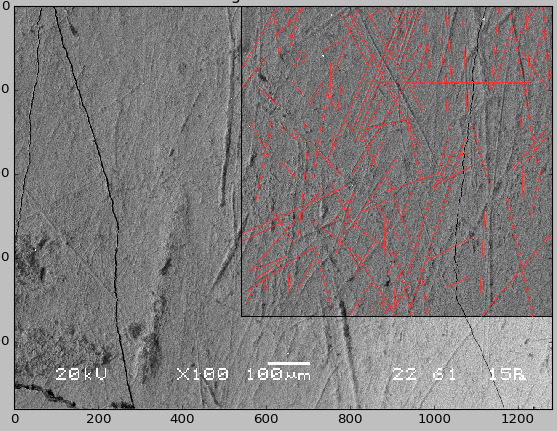
\includegraphics[width=0.65\textwidth]{FigureCanvas}
\caption{FigureCanvas de la imagen}
\label{fig:5.12}
\end{figure}


\subsubsection{Pestañas}
Sección de la imagen donde estarán implementadas las funcionalidades para visualizar las líneas que son detectadas por el algoritmo en la imagen \ref{fig:5.13}.
\begin{itemize}
\item El modo primero es la detección de los surcos en rojo en los dientes 
\item El modo segundo es la corrección/detección manual de las líneas por una persona y quedando reflejadas en la imagen.
\item El modo tercero es la ultima parte del proyecto que consistirá en hacer todo el proceso anterior de forma automática.
\end{itemize}

\begin{figure}[h]
\centering
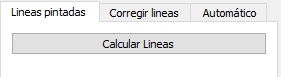
\includegraphics[width=0.65\textwidth]{Pestanas}
\caption{Pestañas}
\label{fig:5.13}
\end{figure}

\section{Diseño procedimental}
En este apartado se van a explicar los pasos que siguen los distintos modos de la aplicación.

\begin{itemize}
	\item Modo semiautomático:
La finalidad de este modo de trabajo en nuestra aplicación, servirá para detectar las estrías que previamente se han pintado en alguna imagen. Para extraer las características de estas.
	\begin{itemize}
		\item Comienza cuando el usuario cargue la imagen en la aplicación.
		\item Posteriormente a la carga, el usuario deberá elegir los parámetros que puede modificar, para la ejecución del algoritmo.
		\item Una vez seleccionados los parámetros, podremos continuar mandando ejecutar a la aplicación el algoritmo, para la detección de las estrías pintadas.
		\item Este nos va a devolver un conjunto de segmentos, que se corresponderán con las estrías que contiene la imagen pintadas, las añadirá a la tabla donde podremos editarlas o añadir algunas que podría no haber detectado dicho algoritmo.
		\item por ultimo podremos guardar las estadísticas, las imágenes original, pintada, longitudes de los segmentos, ángulos, orientaciones, la tabla rellena en formato \LaTeX para incluir en futuros informes y el fichero de configuración del proyecto.
	\end{itemize}
	\item Modo automático:
	La finalidad de este modo de trabajo de la aplicación, consiste en detectar las estrías de dieta de una imagen en blanco desde el cero. Para extraer características de dichas estrías.
	\begin{itemize}
		\item Primero el usuario deberá cargar una imagen, sin que tenga las estrías pintadas, en la aplicación.
		\item posteriormente, deberá elegir los parámetros disponibles para el modo automático, este consistirá en seleccionar la orientación y la longitud mínima que ignora el algoritmo.
		
		\item Una vez que hayan sido seleccionados se habilitara la función de detección de las estrías. Al ejecutar este algoritmo nos mostrara todas las estrías que detecto en la imagen y nos permitirá mover la región de interés que queremos analizar.
		\item Al mover la región de interés que nos conviene analizar y fijarlo desechara las estrías que no estén contenidas y también los trozos de las detectadas que se salgan fuera de la región.
		\item Por ultimo, el paso anterior nos mostrara en la tabla de edición de los segmentos las estrías que ha detectado, pudiendo modificar o eliminar aquellas que nosotros no consideremos útiles.
		También nos permitirá guardar el proyecto tal y como estaba para obtener las estadísticas y demás datos relevantes de las estrías detectadas.
	\end{itemize}
	\item Modo manual:
	La finalidad de este modo no es otra mas que poder incluir el factor humano en la aplicación y corregir los posibles errores o modificar ciertas estrías que nuestro algoritmo ha detectado.
	\begin{itemize}
		\item Después de cargar cualquier imagen en la aplicación podremos acceder a las funciones de este modo.
		\item Para pintar desde cero una imagen, sin que tenga estrías, podemos hacer clic en el la pestaña de corregir lineas y mover la región de iteres por la imagen en la zona que queremos pintar. 
		\item Dentro de la pestaña, anteriormente mencionada, en el botón con el mismo nombre al hacer clic, la primera vez fijaremos el cuadrado y procederemos a seleccionar el origen y el final de la estría que queremos detectar, Para añadirla simplemente tendremos que clicar sobre el botón añadir punto y esta quedara incluida en la tabla. Para pintar nuevas estrías en una imagen que ya contenga estrías pintadas procederemos de forma similar, pero no podremos mover la región de interés. 
		\item Una vez que tengamos alguna estría pintada en nuestra imagen podremos proceder a guardar las estadísticas y todos los datos relevantes del proyecto, de forma similar a los otros modos.
	\end{itemize}

\end{itemize}

\section{Diseño arquitectónico}

En esta sección del anexo de diseño, vamos a explicar y mostrar de forma general como esta diseñado el proyecto, en cuanto a la distribución de paquetes y los patrones de diseño que hemos aplicado.

\subsection{Diseño de paquetes}

En este punto vamos a hacer una breve descripción de cada paquete y de su contenido dentro de la aplicación.

\begin{itemize}
\item Gui:
Este paquete contendrá todos los elementos gráficos de la aplicación y todos lo que se corresponde con interacción con el usuario.
	\begin{itemize}
	\item Mediadores:
	Este paquete va a contener los mediadores de la interfaz para deslocalizar código y complejidad en esta.
	\end{itemize}
\item Código: Este paquete contendrá todas las clases de cálculo que necesitara la aplicación:
	\begin{itemize}
	\item Estadísticas:
	Este paquete contendrá las clases del cálculo de estadísticas.
	\item Informes:
	Este paquete contendrá la generación del informe \LaTeX
	\item Procesado:
	Este paquete se va a encargar tanto del procesado de la imagen 			como del procesado de los segmentos extraídos hasta conseguir los 		segmentos finales.
	\end{itemize}
\end{itemize}

\begin{figure}[h]
	\centering
	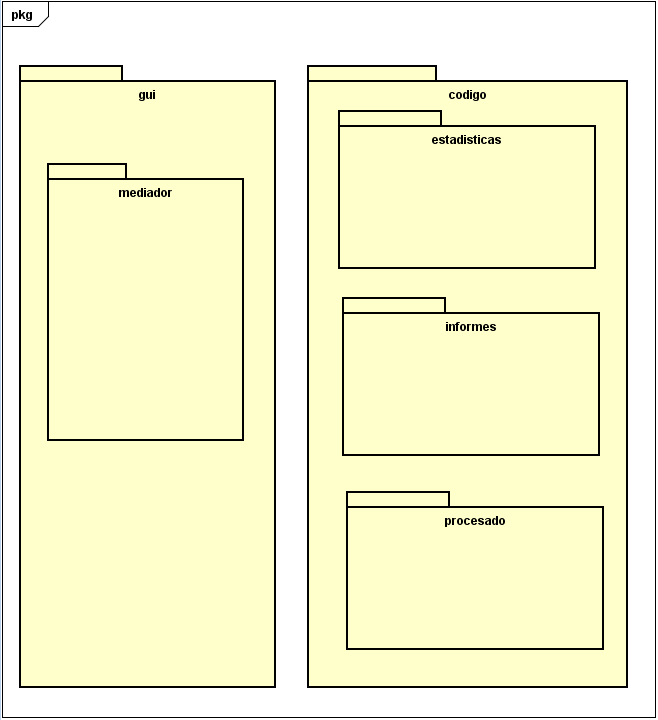
\includegraphics[width=.99\textwidth]{DiaPackages}
	\caption{Diagrama de paquetes inicial}
	\label{fig:C.1.2}
\end{figure}


\subsection{Patrones de diseño}
En este apartado vamos a usar de los patrones de diseño que hemos utilizado en nuestra aplicaron.

El patrón más importante y con el que vamos a empezar es el medidor que consigue hacer que la interfaz este limpia simplemente con las declaraciones de las variables que más adelante va a utilizar.
La base de los patrones de diseño su libro más significativo es \cite{Hunt2013}.

\begin{itemize}
\item Mediador \cite{wiki:Mediador}: Se utiliza para encapsulas las interacciones entre los objetos de la interfaz por lo que se clasifica como patrón de comportamiento.
Como dato curioso, es de los pocos patrones que permiten la bidireccionalidad de comunicación entre las clases, por eso es el patrón idóneo para la interacción de las clases de la interfaz gráfica.
Aplicando este patrón reducimos la dependencia del código por lo que de esta forma las interfaces no ven lo que tienen por debajo y reduce la complejidad.

\textbf{Obtenemos:}
\begin{itemize}
\item Conseguir desacoplamiento.
\item Simplificar y aclarar la comunicación.
\item Centralizar el control.
\item Interfaz simple para un sistema complejo.
\end{itemize}

\item Comando \cite{wiki:Comando}: Se utiliza para encapsular el contenido de una función, así ni el emisor de la operación ni el receptor saber que hay por debajo, pero si poder acceder a las funciones que hay.\\\\
\textbf{Obtenemos:}
\begin{itemize}
\item Permitir la parametrización.
\item Visualizar que ordenes se ejecutan en cada paso.
\item Construir operaciones complicadas a partir de otras más sencillas.
\item Permitir saber que habría que hacer para deshacer una operación.
\end{itemize}
\item Fachada \cite{wiki:Fachada}: Es un patrón de diseño estructural, sirve para reducir la complejidad con la división en clases más pequeñas y reduciendo sus dependencias.\\\\
\textbf{Obtenemos:}
\begin{itemize}
\item Separar en niveles la aplicación.
\item Reducir su complejidad.
\item Desacoplar el código.
\item Interfaz simple para un sistema complejo.
\item Potable y reutilizable.
\end{itemize}
\end{itemize}
